\RequirePackage{docswitch}
% \flag is set by the user, through the makefile:
%    make note
%    make apj
% etc.
\setjournal{\flag}

\documentclass[\docopts]{\docclass}

% You could also define the document class directly
%\documentclass[]{emulateapj}

% Custom commands from LSST DESC, see texmf/styles/lsstdesc_macros.sty
\usepackage{lsstdesc_macros}

\usepackage{graphicx}
\graphicspath{{./}{./figures/}}
\bibliographystyle{apj}

% Add your own macros here:



% ======================================================================

\begin{document}

\title{Covariance Testing}

\maketitlepre

\begin{abstract}

There are a number of codes that compute covariance matrices analytically; the plan is to use these to build TJPCov. In this project, we start along the path of comparing these different codes, building up a suite of tools that can be used to compare covariance matrices. We expect these tools to be useful not only for converging on a single accurate code for computing covariance matrices but also more generally for understanding which parts of the covariance matrix carry the most information (and therefore need the most attention to get right) and which are not relevant (so for example matrices that are not positive definite may still be usable if the negative eigenmodes are not relevant).
\end{abstract}

% Keywords are ignored in the LSST DESC Note style:
\dockeys{}

\maketitlepost

% ----------------------------------------------------------------------
% 

\section{Introduction}
\label{sec:intro}


% ----------------------------------------------------------------------

\section{Methods}
\label{sec:methods}

There are several ways to tests covariance matrices. We will illustrate each of these on cosmic shear statistics $\xi_\pm(\theta)$, focusing for the most part of the Year 1 results of the Dark Energy Survey~\cite{Abbott:2017wau}. One of the codes will be {\tt Cosmolike}~\cite{Krause:2016jvl}; another will be the one used to analyze the KiDS-450 survey~\cite{Kohlinger:2017sxk}.


\subsection{One-to-one Comparison}

This is a simple matter of comparing elements of a covariance matrix, usually starting with diagonal elements. \figref{xipmscatter} shows an example.

\begin{figure}
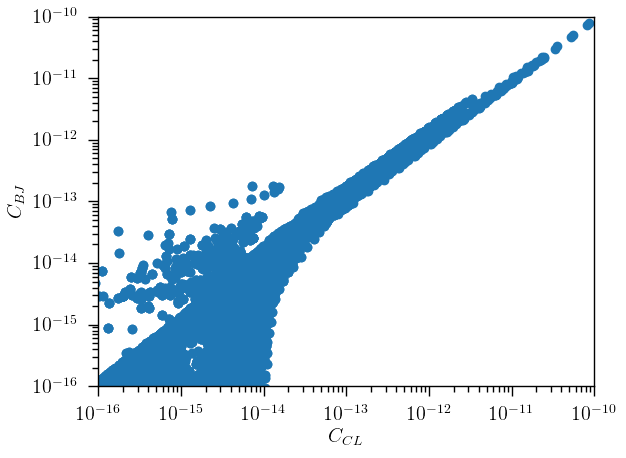
\includegraphics[width=0.9\columnwidth]{xipmscatter.png}
\caption{A simple scatter plot of elements of covariance matrices produced by two separate halo model codes. \label{fig:xipmscatter}}
\end{figure}


\subsection{Eigenvalues and eigenvectors}

This is slightly more sophisticated: diagonalize the covariance matrix and examine the eigenvalues and also the associated eigenvectors. \figref{coveigen} shows an example of the eigenvalues from two different covariance codes.

\begin{figure}
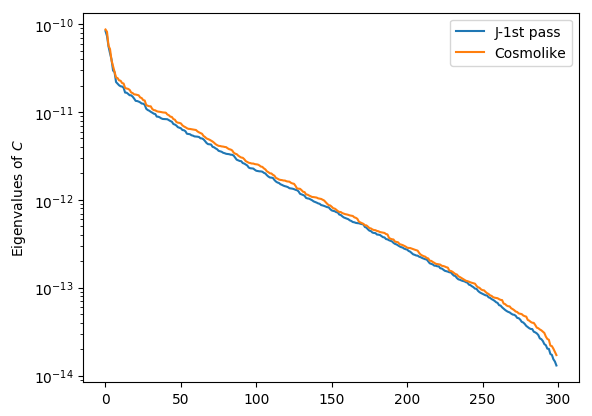
\includegraphics[width=0.9\columnwidth]{coveigen.png}
\caption{A simple scatter plot of elements of covariance matrices produced by two separate halo model codes. \label{fig:coveigen}}
\end{figure}

\figref{evector} shows an example of one of the eigenvectors, the one associated with the smallest eigenvalue. This low-eigenvalue mode picks up the differences between the correlation function at different angular scales (each vertical line delineates between two-point functions of shears in different tomographic bin pairs).

\begin{figure}
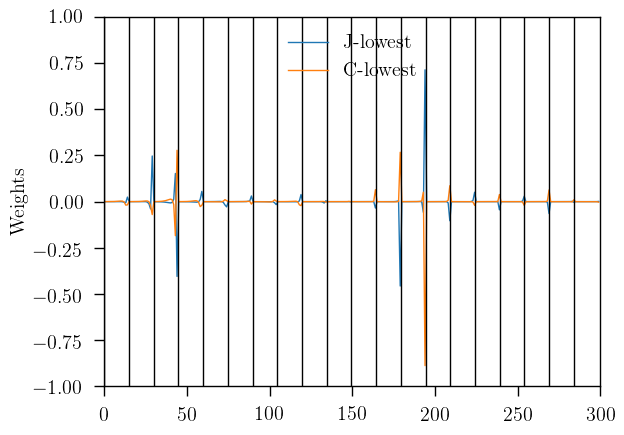
\includegraphics[width=0.9\columnwidth]{evector.png}
\caption{A simple scatter plot of elements of covariance matrices produced by two separate halo model codes. \label{fig:evector}}
\end{figure}

\subsection{Parameter Estimation}

Ultimately, what matters is well the likelihood does at extracting parameter constraints. Since most analyses assume a Gaussian likelihood, this boils down to how well the contours in parameter space agree when using two different covariance matrices.

\subsection{Shrinkage}

There have been several methods proposed in the literature to compress the data vectors, extracting as much information as possible. Here we consider two: first compression at the map level\cite{Alonso:2017hhj}, where linear combination of the tomographic maps are used. If there are 4 tomographic bins, an uncompressed analysis would require ten separate 2-point functions (or 20 for cosmic shear), whereas a compression scheme leads to just a few uncorrelated maps. If there were 3 such maps, then only three 2-point functions would need to be used for the likelihood analysis.

The second compression takes place at the 2-point level\cite{Zablocki:2015zcm}, with the compressed data vector containing linear combinations of the many 2-point functions. In principle, this might work with only $N_p$ 2-point functions where $N_p$ is the number of parameters varied, and each mode, or linear combination, contains all the information necessary about the parameter of interest.


% ----------------------------------------------------------------------

\section{Results}
\label{sec:results}



% ----------------------------------------------------------------------

\section{Discussion}
\label{sec:discussion}



% ----------------------------------------------------------------------

\section{Conclusion}
\label{sec:conclusion}



% ----------------------------------------------------------------------

\subsection*{Acknowledgments}

%%% Here is where you should add your specific acknowledgments, remembering that some standard thanks will be added via the \code{desc-tex/ack/*.tex} and \code{contributions.tex} files.

%This paper has undergone internal review in the LSST Dark Energy Science Collaboration. % REQUIRED if true


 % Standard papers only: author contribution statements. For examples, see http://blogs.nature.com/nautilus/2007/11/post_12.html

% This work used TBD kindly provided by Not-A-DESC Member and benefitted from comments by Another Non-DESC person.

% Standard papers only: A.B.C. acknowledges support from grant 1234 from ...

The DESC acknowledges ongoing support from the Institut National de Physique Nucl\'eaire et de Physique des Particules in France; the Science \& Technology Facilities Council in the United Kingdom; and the Department of Energy, the National Science Foundation, and the LSST Corporation in the United States.  DESC uses resources of the IN2P3 Computing Center (CC-IN2P3--Lyon/Villeurbanne - France) funded by the Centre National de la Recherche Scientifique; the National Energy Research Scientific Computing Center, a DOE Office of Science User Facility supported by the Office of Science of the U.S.\ Department of Energy under Contract No.\ DE-AC02-05CH11231; STFC DiRAC HPC Facilities, funded by UK BIS National E-infrastructure capital grants; and the UK particle physics grid, supported by the GridPP Collaboration.  This work was performed in part under DOE Contract DE-AC02-76SF00515.
 % also available: key standard_short

% This work used some telescope which is operated/funded by some agency or consortium or foundation ...

% We acknowledge the use of An-External-Tool-like-NED-or-ADS.

%{\it Facilities:} \facility{LSST}

% Include both collaboration papers and external citations:
\bibliography{main,lsstdesc}

\end{document}

% ======================================================================
